% Copyright (C) 2018 PUC-Rio/Laboratorio TeleMidia
%
% Permission is granted to copy, distribute and/or modify this document
% under the terms of the GNU Free Documentation License, Version 1.3 or any
% later version published by the Free Software Foundation; with no Invariant
% Sections, with no Front-Cover Texts, and with no Back-Cover Texts. A copy
% of the license is included in the "GNU Free Documentation License" file as
% part of this distribution.

\documentclass[tikz,border=6pt]{standalone}
\usepackage{helvet}
\renewcommand{\familydefault}{\sfdefault}
\usepackage{tikz}
\usetikzlibrary{
  arrows,
  arrows.meta,
  calc,
  math,
  positioning,
}
\begin{document}
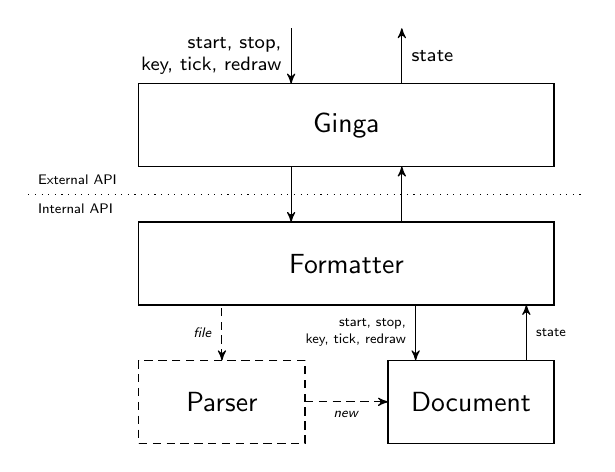
\begin{tikzpicture}[
    node distance=2em,
    x = 2em,
    y = 2em,
    n/.style={
      draw, minimum width=15em, minimum height=3em,
      inner sep=0pt, outer sep=0pt,
    },
    a/.style={>=stealth'},
    b/.style={font=\scriptsize},
    c/.style={font=\tiny},]
  \node[n](Ginga){Ginga};
  \node[n,below=of Ginga](Fmt){Formatter};
  \node[n,below=of Fmt.south west, anchor=north west, minimum width=6em,
  densely dashed]
  (Parser){Parser};
  \node[n,below=of Fmt.south east, anchor=north east, minimum width=6em]
  (Doc){Document};
  %%
  \draw[->,a]($(Ginga.north)+(-1,1)$)
  -- node[b,left,text width=6em, align=right]
  {start, stop,\\key, tick, redraw} ($(Ginga.north)+(-1,0)$);
  %%
  \draw[<-,a]($(Ginga.north)+(1,1)$)
  -- node[b,right,text width=6em] {state} ($(Ginga.north)+(1,0)$);
  %%
  \draw[dotted]
  ($($(Ginga.south west)+(-4,0)$)!.5!(Fmt.north west)$)
  node[c,above,anchor=south west] {External API}
  node[c,below,anchor=north west] {Internal API}
  -- ($(Ginga.south east)!.5!($(Fmt.north east)+(1,0)$)$);
  %%
  \draw[->,a]($(Fmt.north)+(-1,1)$) -- ($(Fmt.north)+(-1,0)$);
  \draw[<-,a]($(Fmt.north)+(1,1)$) -- ($(Fmt.north)+(1,0)$);
  %%
  \draw[<-,a,densely dashed](Parser.north)
  -- node[c,left] {\emph{file}} ($(Parser.north)+(0,1)$);
  \draw[->,a,densely dashed](Parser.east)
  -- node[c,below] {\emph{new}} (Doc.west);
  %%
  \draw[->,a]($(Doc.north)+(-1,1)$)
  -- node[c,left,text width=4em, align=right]
  {start, stop,\\key, tick, redraw} ($(Doc.north)+(-1,0)$);
  \draw[<-,a]($(Doc.north)+(1,1)$)
  -- node[c,right] {state} ($(Doc.north)+(1,0)$);
\end{tikzpicture}
\end{document}
